\input templates/header

\usepackage{epigraph}
\usepackage{listings}
\usepackage{colortbl}

\lstset{
  basicstyle=\ttfamily,
  columns=fullflexible,
		keepspaces=true,
  keywordstyle=\color{red}\bfseries,
  commentstyle=\color{blue},
  showstringspaces=false,
  language=c++,
  tabsize=4,
}

\newcommand{\Sum}{\mathit{sum}}
\newcommand{\MaxSoFar}{\mathit{maxSoFar}}
\newcommand{\MaxEndingHere}{\mathit{maxEndingHere}}

\newcommand*{\RC}[1]{\hfill\makebox[3.0cm][l]{#1}}%


\title[ASD - Introduzione]{\textbf{Algoritmi e Strutture Dati}\\[24pt]Conclusioni}

\graphicspath{{figs/00/}}

\begin{document}

%-------------------------------------------------------------------------
\FrameTitle{}

%-------------------------------------------------------------------------
\begin{frame}{Esame}

\vspace{-9pt}
\begin{myboxtitle}[Esame diviso in due parti]
\BIL
\item \alert{50\% - Parte scritta}
\BI
\item Esame scritto (Uno per modulo/semestre) (Aula)
\item Progetti laboratorio (Uno per semestre) (Homework) 
\EI
\item \alert{50\% - Parte orale}
\EIL
\end{myboxtitle}

\begin{myboxtitle}[Calcolo voto finale x 12 crediti]
\[
\frac{\frac{\textrm{(Voto Scritto 1 + Bonus Lab1)} + \textrm{(Voto Scritto 2 + Bonus Lab2)}}{2} + \textrm{Voto Orale}}{2}
\]
\end{myboxtitle}

\begin{myboxtitle}[Calcolo voto finale x 6 crediti]
\[
\frac{\textrm{Voto Scritto + Bonus Lab + Voto Orale}}{2}
\]
\end{myboxtitle}

\end{frame}

%-------------------------------------------------------------------------
\begin{frame}{Esame scritto}

\vspace{-9pt}
\begin{myboxtitle}[Open-book]
\BI
\item \EE possibile usare libri e appunti, non strumenti elettronici
\EI
\end{myboxtitle}

\begin{myboxtitle}[Regole]
\BI
\item \alert{Salto appello}: in ogni anno solare:
\BI
\item potete \underline{consegnare} al massimo \alert{3} scritti parte A
\item potete \underline{consegnare} al massimo \alert{3} scritti parte B
\EI
\item \alert{Ultimo voto}: se \underline{partecipate} allo scritto del modulo $X$, l'eventuale voto già ottenuto del modulo $X$ viene perso.
\EI
\end{myboxtitle}

\begin{myboxtitle}[Compiti anni passati, con soluzioni]
\small
\url{http://cricca.disi.unitn.it/montresor/teaching/asd/materiale/esercizi/compiti/}
\end{myboxtitle}

\end{frame}

%-------------------------------------------------------------------------
\begin{frame}{Esame orale}

Per accedere all'orale, è necessario:
\BIL
\item Consegnare almeno un progetto funzionante 
\item Ottenere un voto scritto ${} \geq 18$, così definito:

\begingroup
\tiny
\begin{align*}
  \mathrm{12\ crediti} & \qquad \frac{(\textrm{Voto Scritto 1 + BonusLab 1}) + (\textrm{Voto Scritto 2 + BonusLab2 })}{2} \geq 18 \\
  \mathrm{6\ crediti} & \qquad \textrm{Voto Scritto} + \textrm{Bonus Lab} \geq 18 
\end{align*}
\endgroup

\item Dopo aver passato lo scritto, potete venire all'orale nello stesso appello d'esame o in un qualunque appello successivo
\item Se rifiutate un voto all’orale, il voto dello scritto rimane valido
\item Se l'appello è suddiviso in più giornate, non potete rifiutare e pretendere di tornare in una delle giornate successive; dovete passare all'appello (mese) successivo
\EIL
\end{frame}

%-------------------------------------------------------------------------
\begin{frame}{Validità esami}

\vspace{-9pt}
\BB{I voti degli esami scritti non hanno  scadenza}

\medskip
\BB{I voti dei progetti non hanno scadenza}

\medskip
\BB{Caveat emptor!}
\BI
\item Se vi ripresentate fra 10 anni, non garantisco nulla....
\EI

\end{frame}


\begin{frame}{Programma del corso}

\small
\vspace{-18pt}
\begin{columns}[T]
\begin{column}{0.48\textwidth}
\begin{myboxtitle}[Modulo 1]
\BIL
\item Introduzione
	\BI
	\item Analisi degli algoritmi
	\item Notazione asintotica
	\item Ricorrenze
	\item Analisi ammortizzata
	\EI
\item Strutture dati
	\BI
	\item Strutture dati elementari
	\item Alberi
	\item Grafi
	\item Insiemi e dizionari
	\EI
\item Tecniche di risoluzione
	\BI
	\item Divide-et-impera 
  \EI
\EIL
\end{myboxtitle}
\end{column}
\begin{column}{0.52\textwidth}
\begin{myboxtitle}[Modulo 2]
\BIL
\item Strutture dati avanzate
  \BI
  \item Code con priorità 
  \item Insiemi disgiunti 
  \EI
\item Tecniche di risoluzione
  \BI
	\item Scelta struttura dati 
	\item Programmazione dinamica 
	\item Algoritmi greedy
	\item Ricerca locale 
	\item Backtrack
	\item Algoritmi probabilistici
	\EI
\item Problemi intrattabili
	\BI
  \item Algoritmi approssimati
	\item Problemi NP-completi
	\EI
\EIL
\end{myboxtitle}
\end{column}
\end{columns}

\end{frame}


\begin{frame}{Scopo del corso}
\begin{myboxtitle}[Conoscenze e competenze fondamentali]
\BI
\item \alert{Contenuto}: una panoramica aggiornata sui problemi fondamentali e le loro soluzioni
\item	\alert{Metodo}: i principi e le tecniche per risolvere i problemi che capitano nella vita di un programmatore
\EI
\end{myboxtitle}
\TwoColsCustom{0.50}{0.47}{
\BB{Contenuto: elenco di algoritmi}
\BI
\item Analizzate il loro codice
\item Convincetevi che funzionano
\item Provate a implementarli
\EI
}{
\BB{Metodo: pensiero astratto}
\BI
\item Come sviluppare nuovi algoritmi per ogni problema che si presenta
\EI
}
\end{frame}


%-------------------------------------------------------------------------
\begin{frame}{Colloquio di lavoro}
	
\vspace{-9pt}
\begin{myboxtitle}[Problema: Sottovettore di somma massimale]
\BI
\item \textbf{Input}: un vettore di interi $A[1 \ldots n]$
\item \textbf{Output}: il sottovettore $A[i \ldots j]$ di somma massimale,
ovvero il sottovettore la cui somma degli elementi $\sum_{k=i}^j A[k]$ è
più grande o uguale alla somma degli elementi di qualunque altro sottovettore.
\EI
\end{myboxtitle}
\end{frame}


%-------------------------------------------------------------------------
\begin{frame}{La vostra risposta}

\TwoColsCustom{0.60}{0.35}{

\includegraphics[width=\textwidth]{fig0.png}
}{
Eh?  \\(NOOB)
}	

\end{frame}

%-------------------------------------------------------------------------
\begin{frame}{La vostra risposta}
\TwoColsCustom{0.5}{0.45}{
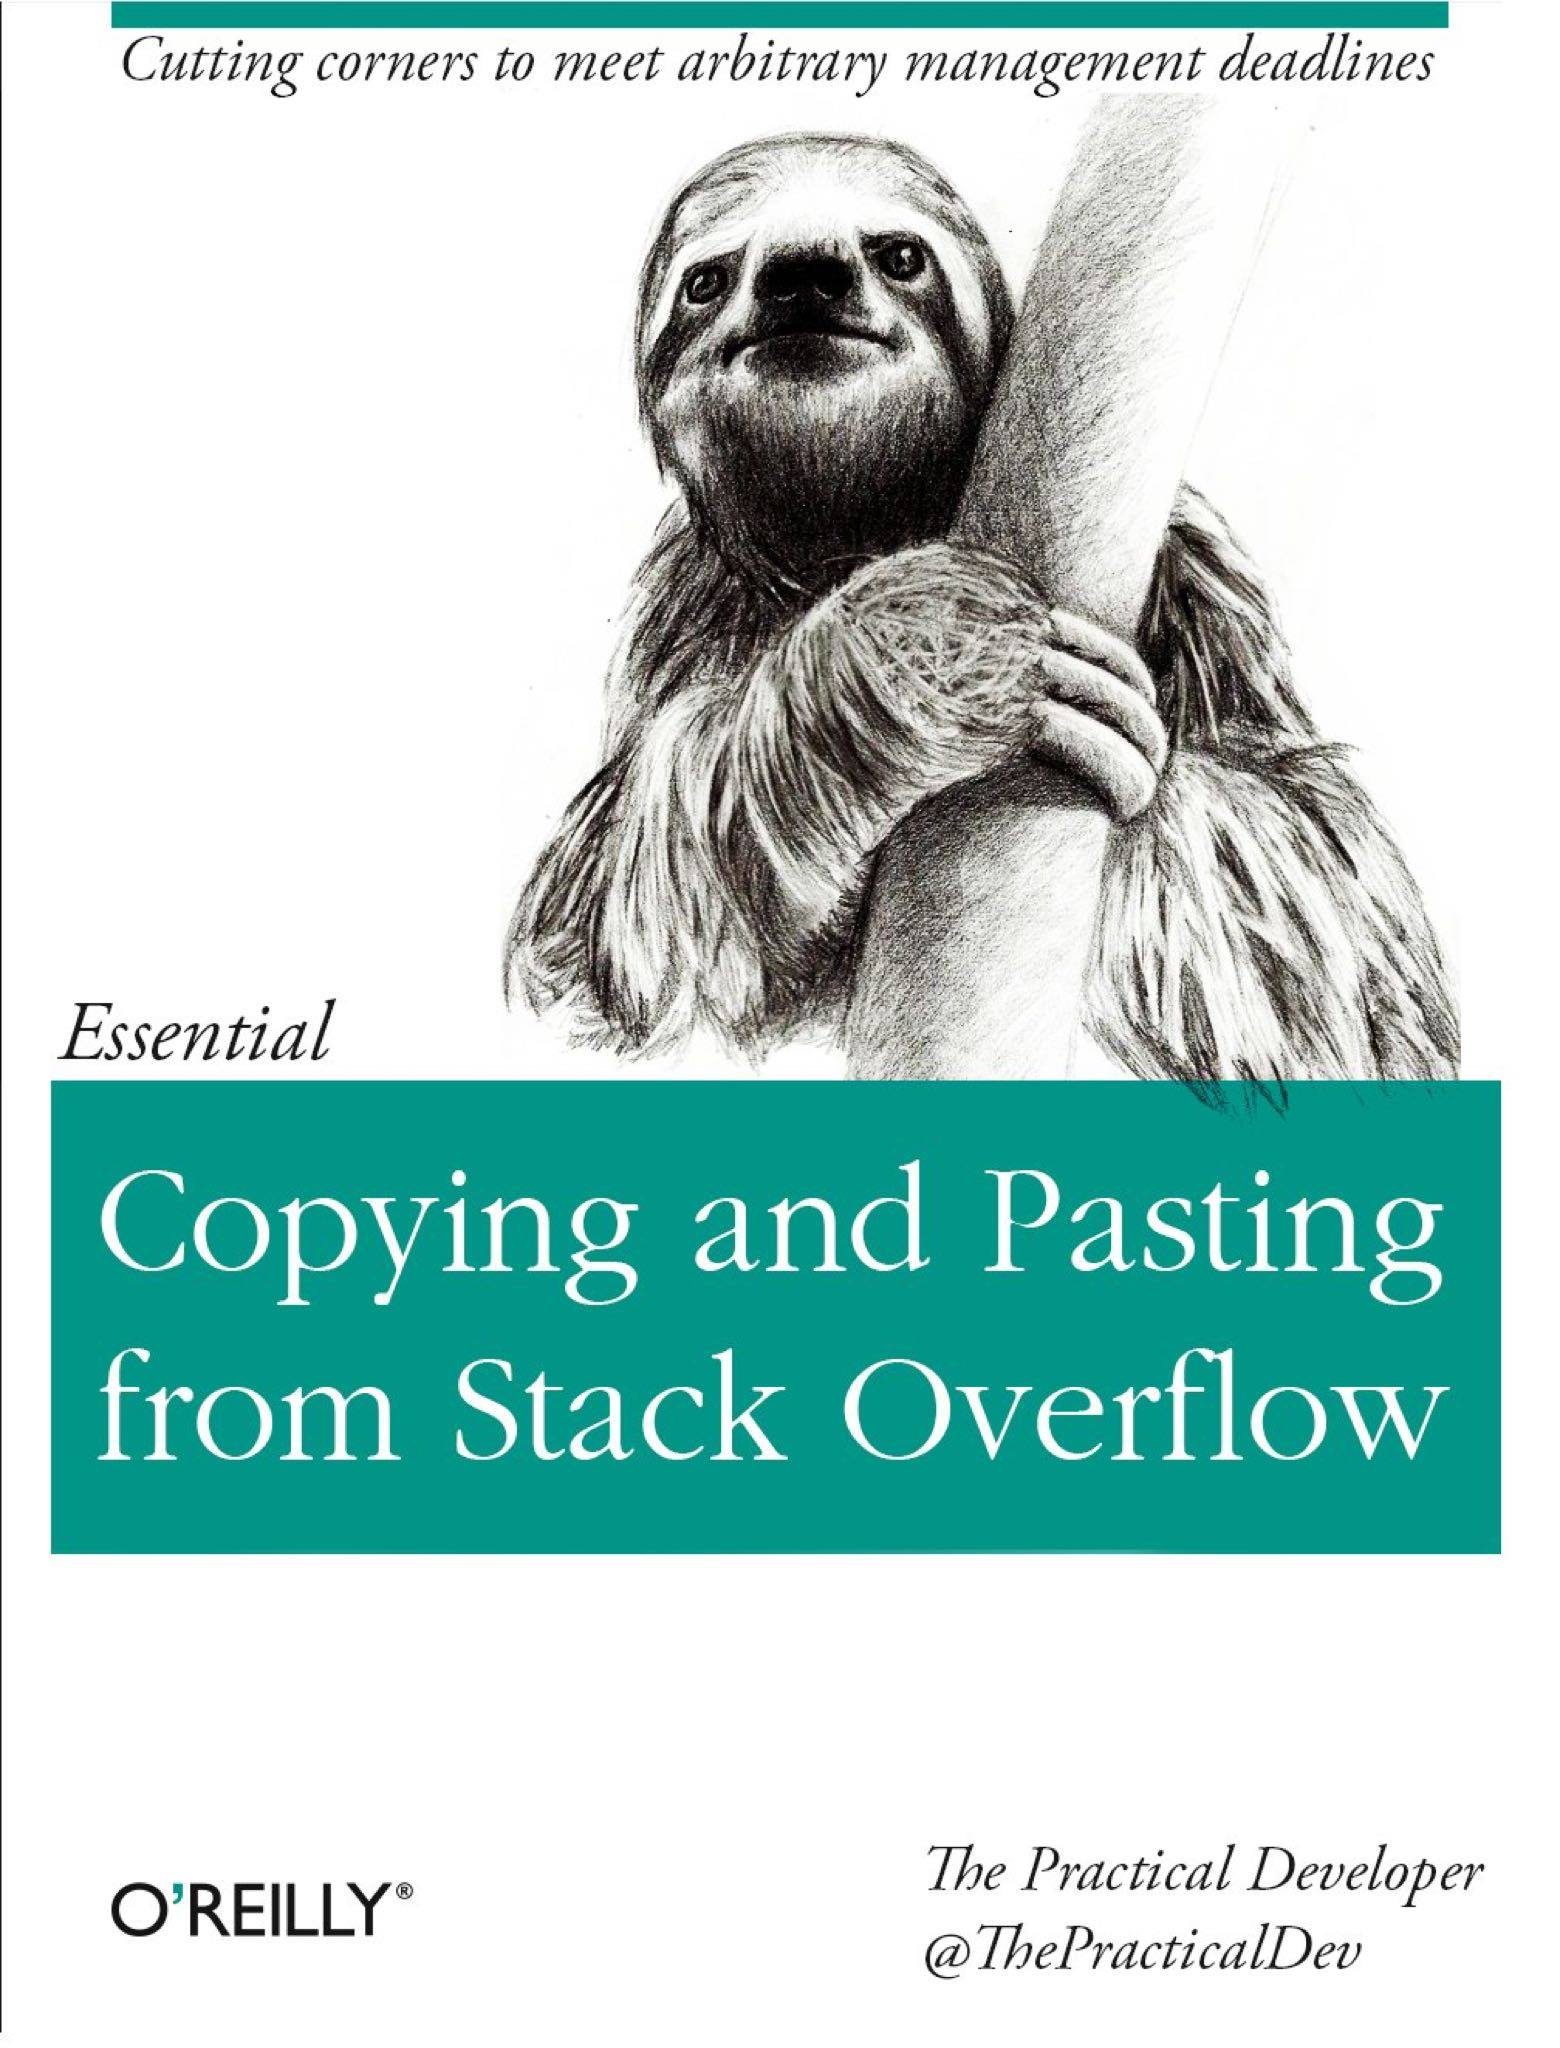
\includegraphics[width=0.8\textwidth]{stackoverflow.jpg}
}{
Posso guardare su StackOverflow?\\(CODE MONKEY)
}

%-------------------------------------------------------------------------
\end{frame}

\begin{frame}{La vostra risposta}
\TwoColsCustom{0.5}{0.45}{
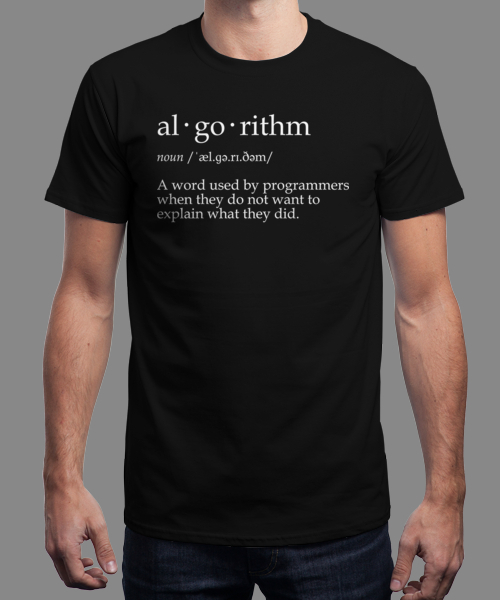
\includegraphics[width=\textwidth]{cs.jpg}
}{
Posso sviluppare un algoritmo efficiente per lei! \\(COMPUTER SCIENTIST)
}	
	
	
\end{frame}


\begin{frame}{Tempi di esecuzione -- Somma massimale}
    
\IG{0.8}{plots.pdf}

\end{frame}

%-------------------------------------------------------------------------
\begin{frame}{Citazioni importanti}

\begin{mdframed}[style=mybox]
\small
"Se volete fare gli scrittori, ci sono due esercizi fondamentali: leggere molto
e scrivere molto. Non conosco stratagemmi per aggirare questa realtà, non
conosco scorciatoie. 

\bigskip
[...]

\bigskip
Quello che voglio dire è che per scrivere al meglio delle proprie capacità, è 
opportuno costruire la propria cassetta degli attrezzi e poi sviluppare i
muscoli necessari a portarla con sè. Allora, invece di farsi scoraggiare
davanti a un lavoro che si preannuncia complicato, può darsi che abbiate a
disposizione l'utensile adatto con il quale mettervi immediatamente all'opera."
\end{mdframed}

\begin{flushright}
On writing, Stephen King
\end{flushright}

\bigskip
{\tiny
\url{http://cricca.disi.unitn.it/montresor/teaching/asd/la-cassetta-degli-attrezzi/}
}

\end{frame}

%-------------------------------------------------------------------------
\begin{frame}{Sull'uso di portatili e cellulari durante la lezione}
	
\vspace{-6pt}
\begin{center}

\includegraphics[width=1.0\textwidth]{attention.png}
\end{center}

\footnotesize
\BI
\item C. Stothart, A. Mitchum, C. Yehnert. \alert{The attentional cost of receiving a cell phone notification}. J Exp Psychol Hum Percept Perform. 41(4):893-7 (Aug. 2015).
\url{https://www.ncbi.nlm.nih.gov/pubmed/26121498}

\item A.F. Ward, K. Duke, A. Gneezy, and M.W. Bos. 
\alert{Brain Drain: The Mere Presence of One’s Own Smartphone Reduces Available Cognitive Capacity}. 
Journal of the Association for Consumer Research, 2(2):140-154 (April 2017) \\
\url{https://www.journals.uchicago.edu/doi/10.1086/691462}

\EI

\end{frame}


%-------------------------------------------------------------------------
\begin{frame}{Varie ed eventuali}
    
\vspace{-12pt}
\TwoColsCustom{0.47}{0.51}{
\begin{myboxtitle}[Opportunità]
\BIL
\item ACM-ICPC
\item Google Summer of Code
\item Google HashCode
\item Hackathon(s)
\item Speck\&Tech
\item Facoltiadi
\item Olimpiadi dell'Informatica
\EIL
\end{myboxtitle}
}{
\begin{myboxtitle}[Google Summer of Code]
\footnotesize
\BI
\item Antonio Quartulli (2011) 
\item Federico Scrinzi (2012) 
\item Pietro Zambelli (2012)
\item Edo Monticelli (2012)
\item Savita Seetaraman (2014)
\item Emilio Dorigatti (2015)
\item Andrea Nardelli (2016)
\item Lodovico Giarretta (2016)
\item Giovanni De Toni (2017)
\item Francesco Gazzetta (2018)
\item Simone Degiacomi (2019)
\EI
\end{myboxtitle}
}

\end{frame}

%-------------------------------------------------------------------------
\begin{frame}{E poi?}

\BB{La mia porta è sempre aperta (tranne quando è chiusa)}
\BIL
\item Prima dell'esame: Non esitate a chiedere un ricevimento
\item Dopo dell'esame: sono sempre a disposizione
  \BI
  \item Se avete un problema algoritmico, fatemi sapere!
  \item Se avete un problema accademico, fatemi sapere!
  \item Se avete un problema personale, beh non esageriamo!
  \EI
\item Tenuto conto dei miei limiti temporali, sono sempre interessato a sapere cosa fate
\EIL

\end{frame}

%-------------------------------------------------------------------------
\begin{frame}{E poi?}

\BB{La mia visione sull'insegnamento}
\BI
\item Se vuoi davvero comprendere qualcosa, insegnala (Yogi Bhajan)
\item Non ci sono maestri, solo allievi (Linus Torvalds)
\EI

\BB{Vi interessa?}
\BIL
\item Tutorato
\item Coderdojo
\item Laboratory of Computer Science Education
\EIL

\end{frame}

%-------------------------------------------------------------------------
\begin{frame}{Chi sono? Cosa hanno in comune?}

\TwoCols{
\begin{center}
\IG{0.8}{foto1.jpg}
\end{center}
}{
\begin{center}
\IG{0.8}{foto2.jpg}
\end{center}
}

\end{frame}

%-------------------------------------------------------------------------
\begin{frame}{Chi sono? Cosa hanno in comune?}

\Huge
\BB{All questions answered!}

\BB{Mercoledì 29 Maggio}

\end{frame}




\end{document}